%%% template.tex
%%%
%%% This LaTeX source document can be used as the basis for your technical
%%% paper or abstract. Regardless of the length of your document, the commands
%%% are all the same.
%%% 
%%% The "\documentclass" command is the first command in your file. If you want to 
%%% prepare a version of your article with line numbers - a "review" version - 
%%% include the "review" parameter:
%%%    \documentclass[review]{acmsiggraph}
%%%
\documentclass[review]{acmsiggraph}

%%% packages and user defined commands
%%% packages
\usepackage{graphicx}
\usepackage{amsmath}
\usepackage{amsfonts}
\usepackage{color}
\usepackage{algorithm}
\usepackage{algorithmic}
%\usepackage{algorithm2e}
% Use Input in the format of Algorithm
%\renewcommand{\algorithmicrequire}{\textbf{Input:}}  
% Use Output in the format of Algorithm
%\renewcommand{\algorithmicensure}{\textbf{Output:}} 
%%% user defined command
\newcommand{\bfd}{{\bf d}}
\newcommand{\bfp}{{\bf p}}
\newcommand{\bfq}{{\bf q}}
\newcommand{\bfc}{{\bf c}}
\newcommand{\bfh}{{\bf h}}
\newcommand{\bfo}{{\bf o}}
\newcommand{\bfn}{{\bf n}}
\newcommand{\bfv}{{\bf v}}

\newcommand{\refEq}[1]{Equation \ref{#1}}
\newcommand{\refSec}[1]{Section \ref{#1}}
\newcommand{\refTab}[1]{Table \ref{#1}}
\newcommand{\refFig}[1]{Figure \ref{#1}}
\newcommand{\refFigs}[1]{Figures #1}

\newcommand{\Ignore}[1]{}
\newcommand{\XGTODO}[1]{\textcolor{red}{{\bf TODO (XGLiu):} #1}}

\newcommand{\Equation}[1]{
	\begin{equation}
		#1
	\end{equation}
}

\newcommand{\Figure}[3]{
  \begin{figure}[thb]
  \centering
  {#2} % comment this line to skip images
  \caption{#3}
  \label{#1}
  \end{figure}
}

\newcommand{\WideFigure}[3]{
  \begin{figure*}[thb]
  \centering
  {#2} % comment this line to skip images
  \caption{#3}
  \label{#1}
  \end{figure*}
}

\newcommand{\Table}[3]{
  \begin{table}[thb]
  \centering
  {#2}
  \caption{#3}
  \label{#1}
  \end{table}
}



%%% Title of your article or abstract.

\title{Completion and Filtering of Incident Light Field for Global Illumination}

\author{Yuchi Huo\thanks{e-mail:}\\Zhejiang University}
\pdfauthor{Yuchi Huo}

%%% Used by the ``review'' variation; the online ID will be printed on 
%%% every page of the content.

\TOGonlineid{45678}

% User-generated keywords.

\keywords{ray tracing, global illumination, incident light field, monte carlo integration, matrix completion}

%%% The next five lines define the rights management block on the first page.
%%% Replace them with the LaTeX commands provided when the form has been completed.

\CopyrightYear{2017}
\setcopyright{acmcopyright}
\conferenceinfo{ACM SIGGRAPH}{MONTH, DAY, and YEAR} 
\isbn{THIS-IS-A-SAMPLE-ISBN}\acmPrice{\$15.00}
\doi{http://doi.acm.org/THIS/IS/A/SAMPLE/DOI}

%%% Start of the document.

\begin{document}

%%% This is the ``teaser'' command, which puts an figure, centered, below 
%%% the title and author information, and above the body of the content.

 \teaser{
   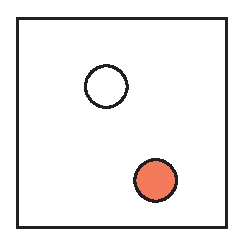
\includegraphics[height=1.5in]{images/samplefigure.eps}
   \caption{This is my teaser.}
 }

\maketitle

\begin{abstract}

This paper presents a new algorithm to reconstruct the incident light field in Monte Carlo ray tracing that improves the image quality by reducing the noise under the same sampling rate of the incident light field and consequently accelerates the speed. The reconstruction is achieved by two interleaved operations -- completion and filtering -- in a low rank sparse matrix completion framework. 

\end{abstract}

% The code below should be generated by the tool at
% http://dl.acm.org/ccs.cfm
% Please copy and paste the code instead of the example below. 
%
\begin{CCSXML}
<ccs2012>
<concept>
<concept_id>10010147.10010371.10010372.10010374</concept_id>
<concept_desc>Computing methodologies~Ray tracing</concept_desc>
<concept_significance>500</concept_significance>
</concept>
</ccs2012>
\end{CCSXML}

\ccsdesc[500]{Computing methodologies~Ray tracing}
%
% End generated code
%

% The next three commands are required, and insert the user-generated keywords, 
% The CCS concepts list, and the rights management text.
% Please make sure there is a blank line between each of these three commands.

\keywordlist

\conceptlist

\printcopyright

\section{Introduction}
As a long standing problem in global illumination,
\section{Related Work}

\section{Light Field Sampling}
We assume the direct illumination is computed separately, and omit it in the algorithm description. 

The radiance $L$ from point $\bfp$ to the camera $\bfc$ can be computed by the following integral over all incident directions:
\Equation{\nonumber
	L_o(\bfp) = \frac{1}{\pi} \int L(\bfp, \omega) f_r(\bfp, \omega_\bfc, \omega) \cos\theta \bfd\omega,
}
where $L(\bfp \leftarrow \omega)$ is the incident light at point $p$ from direction $\omega$, $\omega_\bfc$ is the reflection direction (i.e, the direction from $\bfp$ to $\bfc$), $f_r(\bfp,\omega_\bfc\leftarrow\omega)$ is the BRDF at point $p$.

Suppose that the hemisphere of the incident direction is divided into a set of disjoint subsets: $H = \bigcup_{j=1}^N B_j$, and let $L_{o,j}$ be the integrated illumination of the light passing through $B_i$, i.e.,
$$L_{o,i} = \frac{1}{\pi} \int_{B_i} L(\bfp \leftarrow \omega) f_r(\bfp, \omega_\bfc \leftarrow \omega) \cos\theta \bfd\omega, $$ 
then we have:
\Equation{\nonumber
	L_o(\bfp\rightarrow\bfc)=\sum_{i=1}^N L_{o,i}.
}

To compute the partial illumination result $L_{o,j}$, we can a path tracer, as illustrated as follows: 

\begin{algorithm}[h]
\begin{algorithmic}[1]
	\STATE Input: $B_1\ldots B_N$ -- subdivided hemisphere blocks\;
	\STATE ~~~~~~~~~~~$\bfp$ -- the surface point of a pixel\;
	\STATE ~~~~~~~~~~~$m$ -- a sampling number for the incident rays\;
	\STATE Output: $L_{o,1}\ldots L_{o,N}$ -- partial illuminations\; 
	\STATE ~~~~~~~~~~~~~$\Omega(1)\ldots \Omega(N)$ -- sampling flags for blocks\;
	\FOR{$j \in [1\ldots n]$} 
		\STATE $L_{o,j} \leftarrow 0$, ~~~~$\Omega(j)\leftarrow 0$
	\ENDFOR
	\FOR{ $k\in[1\ldots m]$ }
		\STATE sample a random direction $\omega$ over the hemisphere with $f_r(p,\omega_c,\omega)\cos\theta$ as the pdf \;
		\STATE generate a ray in direction $\omega$ \;
		\STATE compute its incident radiance $L_{in}(\bfp,\omega)$ using path tracer \;
		\STATE find the index $j$ that $\omega\in B_j$ \;
		\STATE $L_{o,j} \leftarrow L_{o,j} + L_{in}(\bfp, \omega)$, ~~~~ $\Omega(j) \leftarrow 1$ \;
	\ENDFOR
\end{algorithmic}
\caption{Sampling procedure for the partial illumination.}
\label{alg:sampling}
\end{algorithm}

\paragraph{Parameterization}


\paragraph{Light Field Sampling}
For two different points $\bfp_1$ and $\bfp_2$, the incident light $L(\bfp_1,\omega)$ and$L(\bfp_2,\omega)$ may be not parallel as the direction parameter $\omega$ are in the points' local coordinate frame.

\section{Light Field Reconstruction}

\subsection{Rank-One Matrix Pursuit}

It is well-know that any matrix ${\bf X}\in\mathfrak{R}^{n\times m}$ can be writting as a linear combination of rank-one matrices, that is:
\Equation{
	{\bf X}={\bf M}(\boldsymbol\theta)=\sum\theta_i{\bf M}_i
}
where $\{ {\bf M}_i\}$ is the set of all $n\times m$ rank-one matrices with unit Frobenius norm.

The original low ran matrix approximation rpoblem aims to minimize the zero normal of $\theta$ subject to the constraint
\begin{eqnarray}
	& \min_{\boldsymbol\theta} \|\boldsymbol\theta\|_0 \\
	s.t. & P_\Omega(\bf M(\boldsymbol\theta)) = P_\Omega(\bf X)
\end{eqnarray}

We filter the bases using cross-bilateral filters

\Equation{\nonumber
	L(\bfp)=\frac{\sum_{\bfq \in {\bf w}}w(\bfp,\bfq)L(\bfq)}
	{\sum_{\bfq \in {\bf w}}w(\bfp,\bfq)}
}%%% end equation
where $\bf w$ denotes a small box window centered at pixel $\bfp$. The size of the window will be discussed later. \XGTODO{where?} And the weighting coefficients $w(\bfp,\bfq)$ are defined by the distances of some feature vectors as follows:
\Equation{\nonumber
	w(\bfp,\bfq)=\Pi_{f}\exp\{-\frac{dist(f_\bfp,f_\bfq)}{2\sigma_f^2}\} 
}%%% end equation
where $f$ denotes a feature vector defined on the image, and $\sigma_f$ a parameter for the variance of feature vecotr $f$. For each pixel in the image, we consider three features: normal vector, position coordinates, and reflectance texture (if any). \XGTODO{Do we really need texture?}

For the feature of normal vector, the variance parameter $\sigma_{normal}$ is computed as $E[\|{\bf n}-E[{\bf n}] \|^2]$, where $\bf n$ denotes the variable of the normal vector.For the position and the texture, the variance parameter $\sigma_{position}$ and $\sigma_{texture}$ are computed in a similar way as the normal. 

As the filter window is halved, the variance parameter $\sigma_{position}$ is multiplied by $1/4$, but $sigma_{normal}$ and $sigma_{texture}$ are kept unchanged.

\section{Implementation Details}

Since the reflection distributions of most materials have a shape similar to phong lobe, we re-parameterize the incident direction $\omega$ using the reflection vector of $\bfp\rightarrow\bfc$, i.e., the elevation angle of the incident direction changes to the angle between $\omega$ and the reflection vector. In this way, the incident light with the equal elevation angle will have similar importance, and helps the sampling scheme for the incident light field  in turn (see \refSec{sec:sampling}).
\section{Experimental Results}

\section{Discussion}

The presented algorithm handles only indirect illumination, and leaves the direct illumination to a separately computation. For point light sources, the direct illumination can be more effectively and efficiently computed by ray casting and using GPU. On the contrary, for area light sources with general shape and intensity distribution, it requires dense sampling to faithfully compute the direct illumination. For the same reason, the proposed algorithm cannot handle caustics effects.

\section*{Acknowledgements}

%%%%%%%%%%%%%%%%%%%%%%%%%%%%%%%%%%%%%%%%%%%%%%%%%%%%%%%%%%%%%%%%%%%
\bibliographystyle{acmsiggraph}
\nocite{*}
\bibliography{rendering}
%%%%%%%%%%%%%%%%%%%%%%%%%%%%%%%%%%%%%%%%%%%%%%%%%%%%%%%%%%%%%%%%%%%
\end{document}
%%%%%%%%%%%%%%%%%%%%%%%%%%%%%%%%%%%%%%%%%%%%%%%%%%%%%%%%%%%%%%%%%%%
\begin{table}[ht]
  \centering
  \caption{A simple table.}
  \begin{tabular}{|r|l|}
    \hline
    7C0 & hexadecimal \\
    3700 & octal \\ \cline{2-2}
    11111000000 & binary \\
    \hline \hline
    1984 & decimal \\
    \hline
  \end{tabular}
\end{table}
  
	\begin{algorithm}[h]
	\begin{algorithmic}[1]
		\FORALL{ $j \in [1\ldots n]$ } 
		\STATE $L_{o,j} \leftarrow 0$, $\Omega(j)\leftarrow 0$
		\ENDFOR
		\FORALL{ $k\in[1\ldots m]$ }
		\STATE sample a random direction $\omega$ over the hemisphere with pdf $f_r(p,\omega_c,\omega)\cos\theta$.
		\STATE sample the incident light from direction $\omega$ 
		\STATE compute its radiance $L_{in}(\bfp,\omega)$ using path tracer.
		\STATE find the index $j$ that $\omega\in B_j$.
		\STATE $L_{o,j} \leftarrow L_{o,j} + L_in(\bfp, \omega)$
		\STATE $\Omega(j) \leftarrow 1$
		
		\ENDFOR
		\STATE 
		\STATE repeat
	\end{algorithmic}
	\caption{Monte Carlo sampling of the partial illuminations.}
	\label{alg:sampling:parital}
\end{algorithm}

\begin{algorithm}[h]
	\STATE Input: $B_1\ldots B_N$ -- subdivided hemisphere blocks\;
	\STATE $\bfp$ -- the surface point of a pixel\;
	\STATE $m$ -- a sampling number for the incident rays\;
	\KwOut{$L_{o,1}\ldots L_{o,N}$ -- partial illuminations\; ~~~~~~~~~~~~~~~$\Omega(1)\ldots \Omega(N)$ -- sampling flags for blocks\; }
	\For{$j \in [1\ldots n]$} 
	{
		$L_{o,j} \leftarrow 0$, ~~~~$\Omega(j)\leftarrow 0$
	}
	\For{ $k\in[1\ldots m]$ }
	{
		sample a random direction $\omega$ over the hemisphere with $f_r(p,\omega_c,\omega)\cos\theta$ as the pdf \;
		generate a ray in direction $\omega$ \;
		compute its incident radiance $L_{in}(\bfp,\omega)$ using path tracer \;
		find the index $j$ that $\omega\in B_j$ \;
		$L_{o,j} \leftarrow L_{o,j} + L_{in}(\bfp, \omega)$, ~~~~ $\Omega(j) \leftarrow 1$ \;
	}
	\caption{Sampling procedure for the partial illumination.}
	\label{alg:sampling}
\end{algorithm}

\begin{algorithm}[thb]
	\begin{algorithmic}[1]
		\STATE Input: $\bf{Y}_\Omega$ and stopping criterion.
		\STATE Initialize: Set $\bf{X}_0=0$, $\theta^0=0$ and $k=1$.
		\STATE 
		\STATE Repeat
		\STATE   Step 1: Find a pair of top left and right singular vectors $(\bf{u}_k,\bf{v}_k)$ of the observed residual matrix $\bf{R}_k=\bf{Y}_\Omega-\bf{X}_{k-1}$.
		\STATE Filter $\bf{u}_k\rightarrow\bar{\bf{u}}_k$
		\STATE Orthogonalize $\bar{\bf{u}}_k\rightarrow\hat{\bf{u}}_k$
		\STATE If $\|\hat{\bf{u}}-\bar{\bf{u}}\|>0.1\|\bar{\bf{u}}\|$, shift to a filter with smaller window, and come back to line 6
		\STATE $\bf{u}_k\leftarrow\hat{\bf{u}}_k$
		\STATE Update $\bf{v}_k$ that pairs $\bf{u}_k$
		\STATE Step 2: Compute the optimal weights $\alpha^k$ for $\bf{X}_{k-1}$ and $\bf{M}_k$ by solving $\min_{\alpha}\|\alpha_1\bf{X}_{k-1}+\alpha_2(\bf{M}_k)_\Omega-\bf{Y}_\Omega\|^2$.
		\STATE Step 3: Set $\bf{X}_k=\alpha_1^k\bf{X}_{k-1}+\alpha_2^k(\bf{M}_k)_\Omega$; $\theta_k^k=\alpha_2^k$ and $\theta_i^k=\theta_i^{k-1}\alpha_1^k$ for $i<k$; $k\leftarrow k+1$.
		\STATE Until stopping criterion is satisfied
		\STATE  
		\STATE Output: Constructed matrix $\hat{\bf{Y}}=\sum_{i=1}^{k}\theta_i^k\bf{M}_i$.
	\end{algorithmic}
	\caption{Filtered EOR1MP.}
	\label{alg:FEOR1MP}
\end{algorithm}\setlength{\textfloatsep}{5pt}% Remove \textfloatsep
\subsection{Filtering}
